\documentclass[11pt,a4paper]{report}
\usepackage[utf8]{inputenc}
%\usepackage{amsmath}
%\usepackage{amsfonts}
%\usepackage{amssymb}
\usepackage{graphicx}
\usepackage[left=1.00cm, right=1.00cm, top=1.25cm, bottom=1.25cm]{geometry}
\usepackage{cite}
\usepackage{natbib}
\usepackage{booktabs}
\usepackage{listings}
\usepackage{xcolor} % 使用颜色宏包
\renewcommand{\bibname}{References}
\renewcommand{\familydefault}{\rmdefault}
\usepackage[caption=false,font=footnotesize]{subfig}
\newcommand{\tabincell}[2]{\begin{tabular}{@{}#1@{}}#2\end{tabular}}  


%%% Maketitle metadata
\newcommand{\horrule}[1]{\rule{\linewidth}{#1}} 	% Horizontal rule

\title{
	%\vspace{-1in} 	
	\usefont{OT1}{bch}{b}{n}
	\normalfont \normalsize \textsc{School of STEM, Computing \& Software Systems, UWB } \\ [25pt]
	\horrule{0.5pt} \\[0.4cm]
	\huge CSS 534 Assignment 5 \\
	\horrule{2pt} \\[0.5cm]
}
\author{
	\normalfont 								\normalsize
	Yangde Li\\[-3pt]		\normalsize
	\today
}
\date{}


\begin{document}
\maketitle
\tableofcontents
\newpage

\section{Introduction}
This report covers an assignment on implementing Ant Colony Optimization with MpiJava.
\newline

\noindent
This is a compulsory exercise in the course CSS 534 Parallel Programming, given by the school of computing \& software systems at the University of Washington, Bothell in 2018.


\section{Parallelism Techniques}
In this implementation with MpiJava, we mainly focus on two types of parallelism techniques: \textbf{Task} and \textbf{Data} decomposition. For the task decomposition, we split the ants to different computing nodes, thus to accelerate whole computing speed. In every optimization loop, the worker nodes send back the delta pheromone generated by the ants in this iteration to master, then master updates the whole pheromone matrix and scatter it to all workers. Another parallel technique is to make every worker run a complete ACO process and update the pheromone matrix using mean value, this is a way to increase the ants searching space and increase the possibility of finding the best path.
\begin{figure}[!htp]
	\centering
	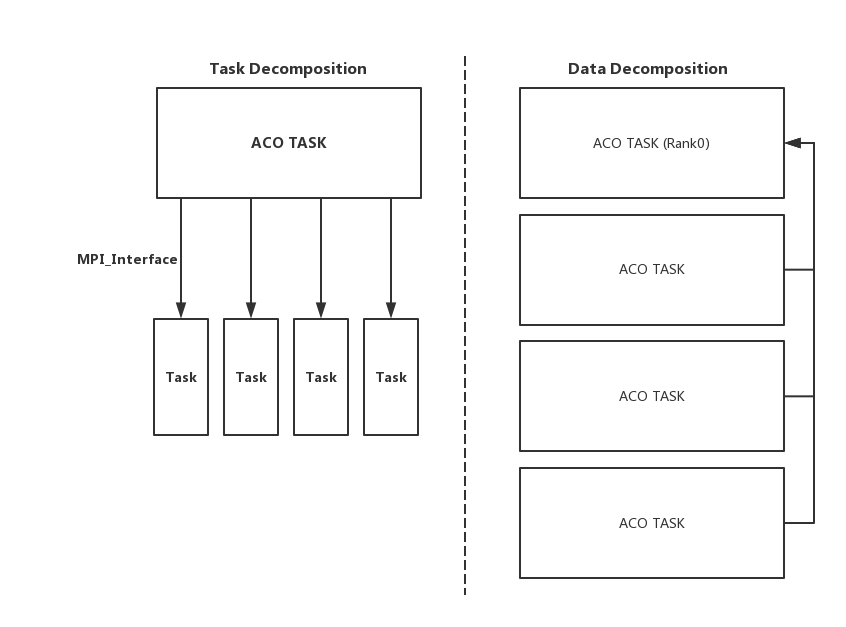
\includegraphics[width=0.8\linewidth]{parallel}
	\caption{Two types of Parallel Pattern}
	\label{fig:parallel}
\end{figure}


\section{Performance Analysis}
For task parallelization, computing task is split into different nodes and the exchanged data is rather small so the performance improvement is obvious. However, the Data Decomposition duplicates the whole data set to run in every node, so the performance improvement should be little.

\section{Programmability Analysis}

\section{Execution Snapshots or Demo with Graphical Results}
\begin{figure}[!htp]
	\centering
	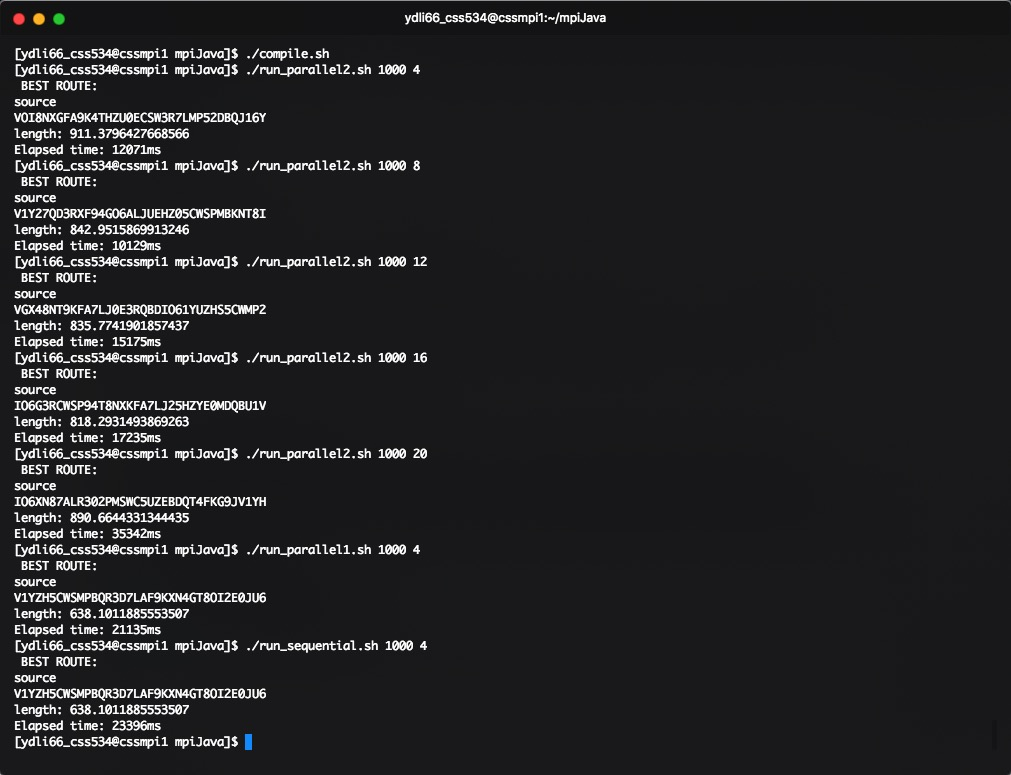
\includegraphics[width=0.7\linewidth]{running}
	\caption{Execution Snapshots}
	\label{fig:running}
\end{figure}





%\begin{lstlisting}
%\end{lstlisting}


%\bibliography{mybib}
%\bibliographystyle{abbrv}
\end{document}